\documentclass[10pt, a4paper, english]{article}\usepackage[]{graphicx}\usepackage[dvipsnames]{xcolor}
% maxwidth is the original width if it is less than linewidth
% otherwise use linewidth (to make sure the graphics do not exceed the margin)
\makeatletter
\def\maxwidth{ %
  \ifdim\Gin@nat@width>\linewidth
    \linewidth
  \else
    \Gin@nat@width
  \fi
}
\makeatother

\definecolor{fgcolor}{rgb}{0.345, 0.345, 0.345}
\newcommand{\hlnum}[1]{\textcolor[rgb]{0.686,0.059,0.569}{#1}}%
\newcommand{\hlstr}[1]{\textcolor[rgb]{0.192,0.494,0.8}{#1}}%
\newcommand{\hlcom}[1]{\textcolor[rgb]{0.678,0.584,0.686}{\textit{#1}}}%
\newcommand{\hlopt}[1]{\textcolor[rgb]{0,0,0}{#1}}%
\newcommand{\hlstd}[1]{\textcolor[rgb]{0.345,0.345,0.345}{#1}}%
\newcommand{\hlkwa}[1]{\textcolor[rgb]{0.161,0.373,0.58}{\textbf{#1}}}%
\newcommand{\hlkwb}[1]{\textcolor[rgb]{0.69,0.353,0.396}{#1}}%
\newcommand{\hlkwc}[1]{\textcolor[rgb]{0.333,0.667,0.333}{#1}}%
\newcommand{\hlkwd}[1]{\textcolor[rgb]{0.737,0.353,0.396}{\textbf{#1}}}%
\let\hlipl\hlkwb

\usepackage{framed}
\makeatletter
\newenvironment{kframe}{%
 \def\at@end@of@kframe{}%
 \ifinner\ifhmode%
  \def\at@end@of@kframe{\end{minipage}}%
  \begin{minipage}{\columnwidth}%
 \fi\fi%
 \def\FrameCommand##1{\hskip\@totalleftmargin \hskip-\fboxsep
 \colorbox{shadecolor}{##1}\hskip-\fboxsep
     % There is no \\@totalrightmargin, so:
     \hskip-\linewidth \hskip-\@totalleftmargin \hskip\columnwidth}%
 \MakeFramed {\advance\hsize-\width
   \@totalleftmargin\z@ \linewidth\hsize
   \@setminipage}}%
 {\par\unskip\endMakeFramed%
 \at@end@of@kframe}
\makeatother

\definecolor{shadecolor}{rgb}{.97, .97, .97}
\definecolor{messagecolor}{rgb}{0, 0, 0}
\definecolor{warningcolor}{rgb}{1, 0, 1}
\definecolor{errorcolor}{rgb}{1, 0, 0}
\newenvironment{knitrout}{}{} % an empty environment to be redefined in TeX

\usepackage{alltt}
%typesetting
\usepackage[margin = 1in]{geometry} % margins
\usepackage[T1]{fontenc} % font encoding
\usepackage{babel} %enables typesetting for multiple languages
\usepackage{parskip} %new lines
\usepackage{graphicx} 
\usepackage{float}
\floatplacement{figure}{H} %when printing tables, include  table.position="H"
\usepackage{bm}
\usepackage{amsmath}
\graphicspath{ {.} }
\usepackage[dvipsnames]{xcolor} % more colors

\usepackage[colorlinks]{hyperref}


 %clickable table of contents from hyperref
\hypersetup{
    colorlinks,
    citecolor=black,
    filecolor=black,
    linkcolor=black,
    urlcolor=black
}

\usepackage[colorinlistoftodos]{todonotes}


\title{Machine Learning 2ST129 26605 HT2023
 Assignment 3}
\author{Anonymous Student}
\date{\today}
\IfFileExists{upquote.sty}{\usepackage{upquote}}{}
\begin{document}
\maketitle
\newpage
\tableofcontents
\newpage




\section*{General Information}
\begin{itemize}
\item Time used for reading 3 hours : 
\item Time used for basic assignment 15 :
\item Time used for extra assignment 3 hours 
\item Good with lab: Good introduction to Keras. Also fun to somewhat freely try to experiment with the model instead of only having to implement a given model. 
\item Things to improve in the lab: Maybe more about if there is some type of general strategy, or at least rough guidelines,  on how to tune a model to get better accuracy. For example, when to implement regularizers on the layers or how to tune the learning rate. Now I just tested it randomly without any specific strategy until i was satisfied with the results. 
\end{itemize}

\begin{knitrout}
\definecolor{shadecolor}{rgb}{0.969, 0.969, 0.969}\color{fgcolor}\begin{kframe}
\begin{alltt}
\hlcom{#Libraries}
 \hlkwd{library}\hlstd{(tidyverse)}
 \hlkwd{library}\hlstd{(xtable)}
 \hlkwd{library}\hlstd{(keras)}
 \hlkwd{library}\hlstd{(tensorflow)}
\end{alltt}
\end{kframe}
\end{knitrout}

\section{Task 1}
\subsection{1.1}
First we instantiate and  visualize the data.
\begin{knitrout}
\definecolor{shadecolor}{rgb}{0.969, 0.969, 0.969}\color{fgcolor}\begin{kframe}
\begin{alltt}
 \hlstd{mnist} \hlkwb{<-} \hlkwd{dataset_mnist}\hlstd{()}
\hlstd{x_train} \hlkwb{<-} \hlstd{mnist}\hlopt{$}\hlstd{train}\hlopt{$}\hlstd{x}\hlopt{/}\hlnum{255}
\hlstd{x_test}\hlkwb{<-} \hlstd{mnist}\hlopt{$}\hlstd{test}\hlopt{$}\hlstd{x}\hlopt{/}\hlnum{255}

\hlcom{#' function to iterate through the different idx and plot the images}
\hlstd{plot_images} \hlkwb{<-} \hlkwa{function}\hlstd{(}\hlkwc{image_array}\hlstd{,} \hlkwc{y}\hlstd{,} \hlkwc{idx}\hlstd{,} \hlkwc{pixel_dim} \hlstd{=} \hlnum{28}\hlstd{,} \hlkwc{ncol} \hlstd{=} \hlnum{3}\hlstd{,} \hlkwc{pred}\hlstd{=}\hlnum{FALSE}\hlstd{) \{}
  \hlkwd{par}\hlstd{(}\hlkwc{mfrow} \hlstd{=}\hlkwd{c}\hlstd{(}\hlnum{4}\hlstd{,}\hlnum{2}\hlstd{))}

  \hlkwa{for} \hlstd{(i} \hlkwa{in} \hlstd{idx) \{}
    \hlstd{im} \hlkwb{<-} \hlstd{image_array[i,,]}
    \hlstd{im} \hlkwb{<-} \hlkwd{t}\hlstd{(}\hlkwd{apply}\hlstd{(im,} \hlnum{2}\hlstd{, rev))}
    \hlkwa{if} \hlstd{(}\hlkwd{isFALSE}\hlstd{(pred))\{}
      \hlstd{main} \hlkwb{<-} \hlkwd{paste}\hlstd{(y[i])}
    \hlstd{\}} \hlkwa{else}\hlstd{\{}
\hlstd{main} \hlkwb{<-} \hlkwd{paste}\hlstd{(}\hlstr{"Actual: "}\hlstd{,} \hlkwd{paste0}\hlstd{(y[i],}\hlstr{","}\hlstd{),} \hlstr{"Predicted:"}\hlstd{, pred[i])}
    \hlstd{\}}
  \hlkwd{image}\hlstd{(}\hlnum{1}\hlopt{:}\hlstd{pixel_dim,} \hlnum{1}\hlopt{:}\hlstd{pixel_dim, im,} \hlkwc{col} \hlstd{=} \hlkwd{gray}\hlstd{((}\hlnum{0}\hlopt{:}\hlnum{255}\hlstd{)}\hlopt{/}\hlnum{255}\hlstd{),}
            \hlkwc{xlab} \hlstd{=} \hlstr{""}\hlstd{,} \hlkwc{ylab} \hlstd{=} \hlstr{""}\hlstd{,} \hlkwc{xaxt} \hlstd{=} \hlstr{'n'}\hlstd{,} \hlkwc{yaxt} \hlstd{=} \hlstr{'n'}\hlstd{,}
        \hlkwc{main} \hlstd{= main)}
  \hlstd{\}}

  \hlkwd{par}\hlstd{(}\hlkwc{mfrow} \hlstd{=} \hlkwd{c}\hlstd{(}\hlnum{1}\hlstd{,} \hlnum{1}\hlstd{))}
\hlstd{\}}
\end{alltt}
\end{kframe}
\end{knitrout}

\begin{knitrout}
\definecolor{shadecolor}{rgb}{0.969, 0.969, 0.969}\color{fgcolor}\begin{kframe}
\begin{alltt}
\hlkwd{plot_images}\hlstd{(}\hlkwc{image_array} \hlstd{= x_train,} \hlkwc{y} \hlstd{= mnist}\hlopt{$}\hlstd{train}\hlopt{$}\hlstd{y,} \hlkwc{idx} \hlstd{=} \hlkwd{c}\hlstd{(}\hlnum{1}\hlopt{:}\hlnum{8}\hlstd{))}
\end{alltt}
\end{kframe}\begin{figure}
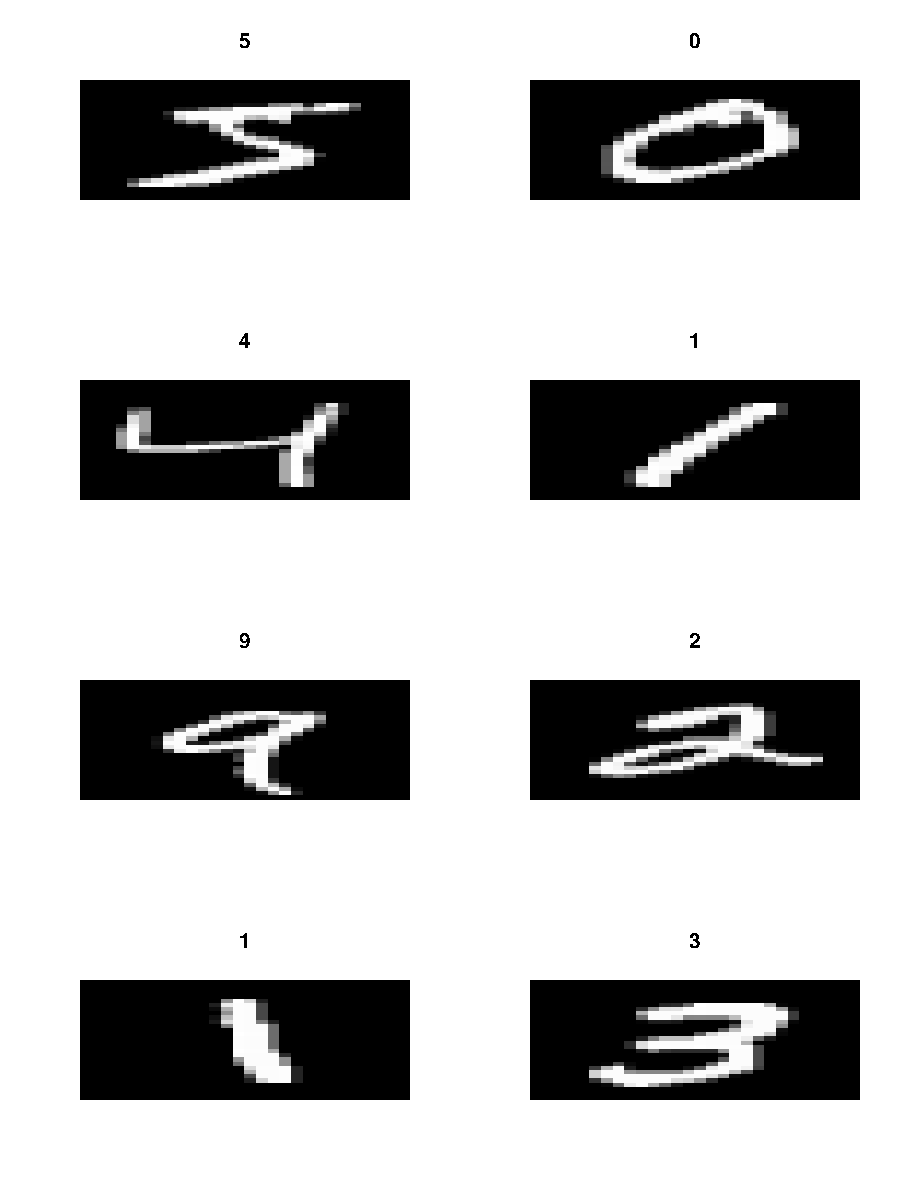
\includegraphics[width=\maxwidth]{figure/images-1} \caption[Visualization of digits]{Visualization of digits}\label{fig:images}
\end{figure}

\end{knitrout}



\subsection{1.2}

The data set contains of 60k 28x28 grayscale images of the 10 digits, as well as a test set with 10k images. 
\begin{knitrout}
\definecolor{shadecolor}{rgb}{0.969, 0.969, 0.969}\color{fgcolor}\begin{kframe}
\begin{alltt}
\hlkwd{str}\hlstd{(mnist}\hlopt{$}\hlstd{train)}
\end{alltt}
\begin{verbatim}
List of 2
 $ x: int [1:60000, 1:28, 1:28] 0 0 0 0 0 0 0 0 0 0 ...
 $ y: int [1:60000(1d)] 5 0 4 1 9 2 1 3 1 4 ...
\end{verbatim}
\begin{alltt}
\hlkwd{str}\hlstd{(mnist}\hlopt{$}\hlstd{test)}
\end{alltt}
\begin{verbatim}
List of 2
 $ x: int [1:10000, 1:28, 1:28] 0 0 0 0 0 0 0 0 0 0 ...
 $ y: int [1:10000(1d)] 7 2 1 0 4 1 4 9 5 9 ...
\end{verbatim}
\end{kframe}
\end{knitrout}



\subsection{1.3}
Now we want to implement a simple-feed-forward neural network with one hidden layer with 16 units and by using the sigmoid activation function. The steps done here to modify the data or model is as proposed by the guide Getting Started with Keras. 


\begin{knitrout}
\definecolor{shadecolor}{rgb}{0.969, 0.969, 0.969}\color{fgcolor}\begin{kframe}
\begin{alltt}
\hlcom{#Since the reponse variablbe y is an vector with integer values with 10 classes,}
\hlcom{# we need to one-hot encode them into binary class matrices}
\hlcom{#}
\hlstd{y_train} \hlkwb{<-} \hlkwd{to_categorical}\hlstd{(mnist}\hlopt{$}\hlstd{train}\hlopt{$}\hlstd{y,} \hlkwc{num_classes} \hlstd{=} \hlnum{10}\hlstd{)}
\hlstd{y_test} \hlkwb{<-} \hlkwd{to_categorical}\hlstd{(mnist}\hlopt{$}\hlstd{test}\hlopt{$}\hlstd{y,} \hlkwc{num_classes} \hlstd{=} \hlnum{10}\hlstd{)}
\end{alltt}
\end{kframe}
\end{knitrout}


\begin{knitrout}
\definecolor{shadecolor}{rgb}{0.969, 0.969, 0.969}\color{fgcolor}\begin{kframe}
\begin{alltt}
\hlcom{# Model architecture}
\hlstd{model} \hlkwb{<-} \hlkwd{keras_model_sequential}\hlstd{(}\hlkwc{input_shape} \hlstd{=} \hlkwd{c}\hlstd{(}\hlnum{28}\hlstd{,}\hlnum{28}\hlstd{))} \hlopt
  \hlkwd{layer_flatten}\hlstd{()} \hlopt
  \hlkwd{layer_dense}\hlstd{(}\hlkwc{units} \hlstd{=} \hlnum{16}\hlstd{,} \hlkwc{activation} \hlstd{=} \hlstr{'sigmoid'}\hlstd{)} \hlopt
  \hlcom{# Hidden layer with 16 units and sigmoid activation}
  \hlkwd{layer_dense}\hlstd{(}\hlkwc{units} \hlstd{=} \hlnum{10}\hlstd{,} \hlkwc{activation} \hlstd{=} \hlstr{'softmax'}\hlstd{)}
\hlcom{# Output layer with softmax activation}
\end{alltt}
\end{kframe}
\end{knitrout}

\begin{knitrout}
\definecolor{shadecolor}{rgb}{0.969, 0.969, 0.969}\color{fgcolor}\begin{kframe}
\begin{alltt}
\hlkwd{print}\hlstd{(model)}
\end{alltt}
\begin{verbatim}
Model: "sequential"
________________________________________________________________________________
 Layer (type)                       Output Shape                    Param #     
================================================================================
 flatten (Flatten)                  (None, 784)                     0           
 dense_1 (Dense)                    (None, 16)                      12560       
 dense (Dense)                      (None, 10)                      170         
================================================================================
Total params: 12730 (49.73 KB)
Trainable params: 12730 (49.73 KB)
Non-trainable params: 0 (0.00 Byte)
________________________________________________________________________________
\end{verbatim}
\end{kframe}
\end{knitrout}
The model has  12730 parameters in total. The input layer has 12560 and the output layer has 170.
Next we compile the model and fit it to compute the validation accuracy. For computational reasons we can set the \texttt{batch\_size} to 128 to make it run faster,  while also setting \texttt{validation\_split()} to 0.2 so that it for every epoch uses 20 percent of the data as validation.  
\begin{knitrout}
\definecolor{shadecolor}{rgb}{0.969, 0.969, 0.969}\color{fgcolor}\begin{kframe}
\begin{alltt}
\hlcom{# Compile the model}
\hlcom{#here we choose the "adam optimizer as well as categorical_crossentropy}
\hlstd{model} \hlopt \hlkwd{compile}\hlstd{(}
  \hlkwc{optimizer} \hlstd{=} \hlstr{'adam'}\hlstd{,}
  \hlkwc{loss} \hlstd{=} \hlstr{'categorical_crossentropy'}\hlstd{,}
  \hlkwc{metrics} \hlstd{=} \hlkwd{c}\hlstd{(}\hlstr{'accuracy'}\hlstd{)}
\hlstd{)}

\hlcom{# Train the model}
\hlcom{#here we choose batch_size = 128 and validaiton split = 0.2}
\hlcom{#the number of samples used in each iteration of gradient descent }
\hlcom{# which is more computationally efficient}
\hlcom{# Validation is the fraction of the training data that is reserved for validation. }

\hlstd{history} \hlkwb{<-} \hlstd{model} \hlopt \hlkwd{fit}\hlstd{(}
  \hlstd{x_train, y_train,}
  \hlkwc{epochs} \hlstd{=} \hlnum{30}\hlstd{,} \hlkwc{batch_size} \hlstd{=} \hlnum{128}\hlstd{,}
  \hlkwc{validation_split} \hlstd{=} \hlnum{0.2}
  \hlcom{#validation_data = list(x_test, y_test)}
\hlstd{)}
\end{alltt}
\end{kframe}
\end{knitrout}
For the last epoch, we have the following results:
\begin{knitrout}
\definecolor{shadecolor}{rgb}{0.969, 0.969, 0.969}\color{fgcolor}\begin{kframe}
\begin{alltt}
epoch 30/30
375/375 [==============================] - 1s 2ms/step 
- loss: 0.1536 - accuracy: 0.9559 - val_loss: 0.1906 - val_accuracy: 0.9438
\end{alltt}
\end{kframe}
\end{knitrout}

Hence the accuracy is 0.956 and the validation accuracy is 0.944. The results is also shown in figure \ref{fig:model1}below
\begin{knitrout}
\definecolor{shadecolor}{rgb}{0.969, 0.969, 0.969}\color{fgcolor}\begin{kframe}
\begin{alltt}
\hlstd{knitr}\hlopt{::}\hlkwd{include_graphics}\hlstd{(}\hlstr{"model1.png"}\hlstd{)}
\end{alltt}
\end{kframe}\begin{figure}
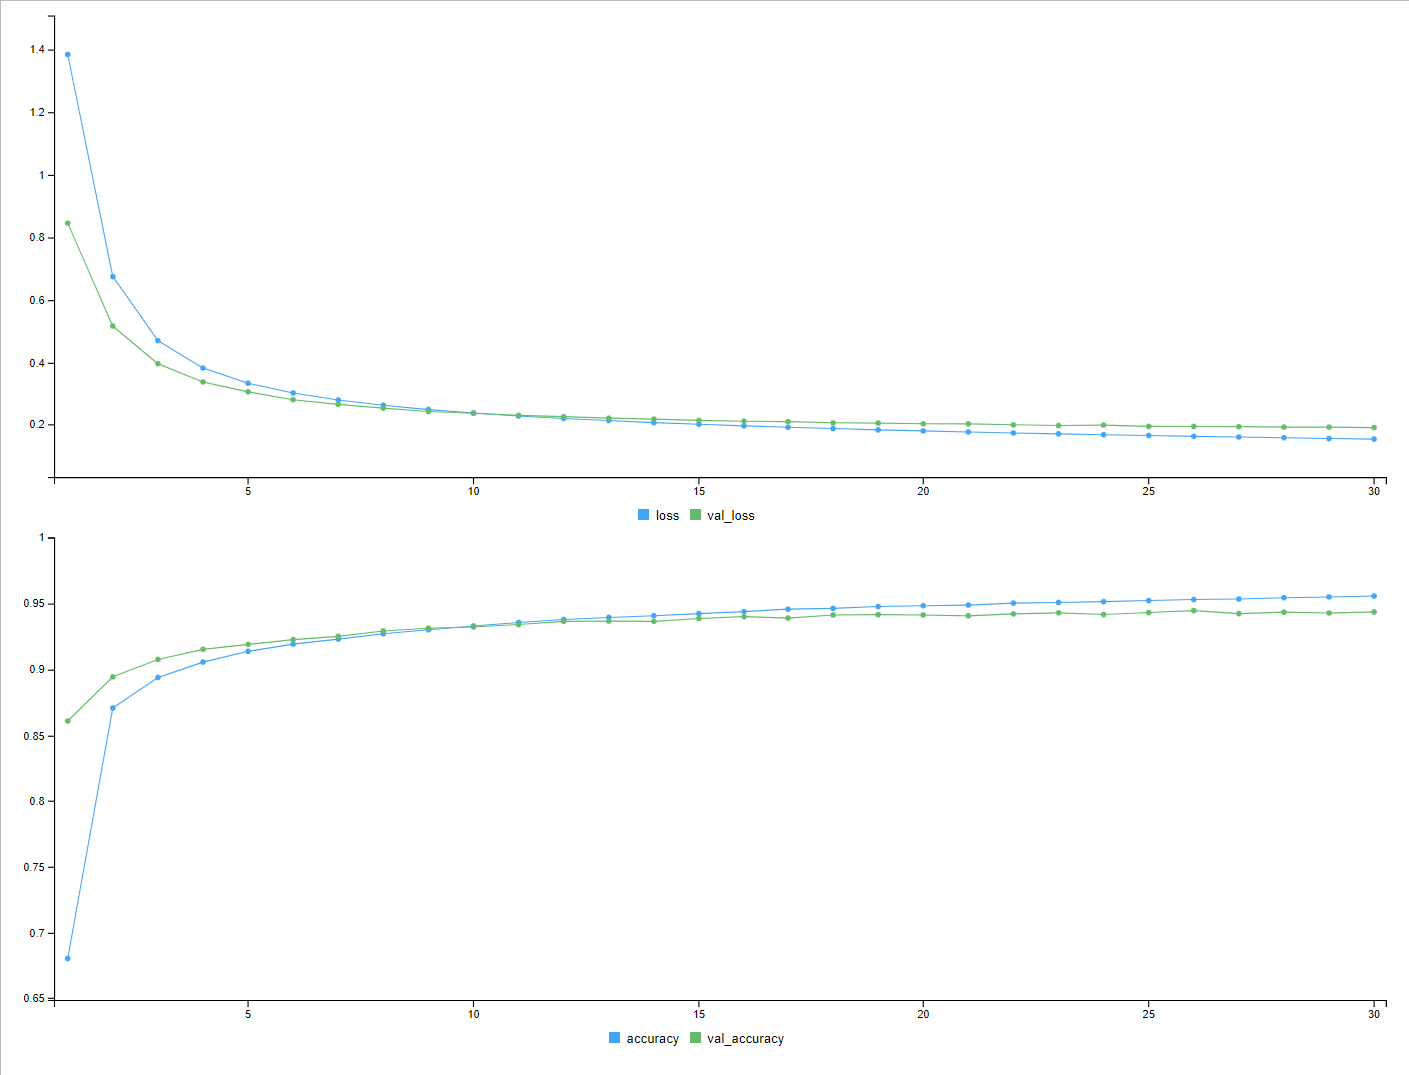
\includegraphics[width=\maxwidth]{model1} \caption[Results for model 1]{Results for model 1}\label{fig:model1}
\end{figure}

\end{knitrout}

\subsection{1.4}
Now we make some adjustments to the model by implementing the following:
\begin{itemize}
\item Increase the number of hidden units to 128.
\item Change the activation function to reLU. 
\item Change the optimizer to RMSprop. 
\item Add a second layer with 128 hidden units. 
\item Add dropout with 0.2 dropout probability for both of  hidden layers. 
\item Add batch normalization for both of hidden layers.
\end{itemize}

\begin{knitrout}
\definecolor{shadecolor}{rgb}{0.969, 0.969, 0.969}\color{fgcolor}\begin{kframe}
\begin{alltt}
\hlcom{# Model architecture}
\hlstd{model_new} \hlkwb{<-} \hlkwd{keras_model_sequential}\hlstd{(}\hlkwc{input_shape} \hlstd{=} \hlkwd{c}\hlstd{(}\hlnum{28}\hlstd{,}\hlnum{28}\hlstd{))} \hlopt
  \hlkwd{layer_flatten}\hlstd{()} \hlopt
  \hlkwd{layer_dense}\hlstd{(}\hlkwc{units} \hlstd{=} \hlnum{128}\hlstd{,} \hlkwc{activation} \hlstd{=} \hlstr{'relu'}\hlstd{)} \hlopt  \hlcom{# Hidden layer with 128 }
  \hlcom{#units and relu activation. More learning capacity but also more overfitting}
  \hlkwd{layer_dropout}\hlstd{(}\hlnum{0.2}\hlstd{)} \hlopt  \hlcom{#dropping out random neurons with p=0.2}
  \hlkwd{layer_batch_normalization}\hlstd{()} \hlopt
  \hlkwd{layer_dense}\hlstd{(}\hlkwc{units}\hlstd{=}\hlnum{128}\hlstd{,} \hlkwc{activation}\hlstd{=}\hlstr{"relu"}\hlstd{)} \hlopt \hlcom{#second layer}
  \hlkwd{layer_dropout}\hlstd{(}\hlnum{0.2}\hlstd{)} \hlopt
  \hlkwd{layer_batch_normalization}\hlstd{()} \hlopt
  \hlkwd{layer_dense}\hlstd{(}\hlkwc{units} \hlstd{=} \hlnum{10}\hlstd{,} \hlkwc{activation} \hlstd{=} \hlstr{'softmax'}\hlstd{)}
\hlcom{# Output layer with softmax activation}

  \hlcom{#batch normalization: reparametrizes the model in a way that introduces both }
  \hlcom{#additive and multiplicative noise on the hidden units at training time}

\hlkwd{summary}\hlstd{(model_new)}
\end{alltt}
\begin{verbatim}
Model: "sequential_1"
________________________________________________________________________________
 Layer (type)                  Output Shape               Param #    Trainable  
================================================================================
 flatten_1 (Flatten)           (None, 784)                0          Y          
 dense_4 (Dense)               (None, 128)                100480     Y          
 dropout_1 (Dropout)           (None, 128)                0          Y          
 batch_normalization_1 (Batch  (None, 128)                512        Y          
 Normalization)                                                                 
 dense_3 (Dense)               (None, 128)                16512      Y          
 dropout (Dropout)             (None, 128)                0          Y          
 batch_normalization (BatchNo  (None, 128)                512        Y          
 rmalization)                                                                   
 dense_2 (Dense)               (None, 10)                 1290       Y          
================================================================================
Total params: 119306 (466.04 KB)
Trainable params: 118794 (464.04 KB)
Non-trainable params: 512 (2.00 KB)
________________________________________________________________________________
\end{verbatim}
\end{kframe}
\end{knitrout}

\begin{knitrout}
\definecolor{shadecolor}{rgb}{0.969, 0.969, 0.969}\color{fgcolor}\begin{kframe}
\begin{alltt}
\hlstd{model_new} \hlopt \hlkwd{compile}\hlstd{(}
  \hlkwc{optimizer} \hlstd{=} \hlstr{'RMSprop'}\hlstd{,}\hlcom{# RMSPROP instead of adam}
  \hlkwc{loss} \hlstd{=} \hlstr{'categorical_crossentropy'}\hlstd{,}
  \hlkwc{metrics} \hlstd{=} \hlkwd{c}\hlstd{(}\hlstr{'accuracy'}\hlstd{)}
\hlstd{)}

\hlstd{history} \hlkwb{<-} \hlstd{model_new} \hlopt \hlkwd{fit}\hlstd{(}
  \hlstd{x_train, y_train,}
  \hlkwc{epochs} \hlstd{=} \hlnum{30}\hlstd{,}\hlkwc{batch_size} \hlstd{=} \hlnum{128}\hlstd{,}
  \hlkwc{validation_split} \hlstd{=} \hlnum{0.2}
\hlstd{)}
\end{alltt}
\end{kframe}
\end{knitrout}

\begin{knitrout}
\definecolor{shadecolor}{rgb}{0.969, 0.969, 0.969}\color{fgcolor}\begin{kframe}
\begin{alltt}
375/375 [==============================] - 2s 4ms/step
- loss: 0.0330 - accuracy: 0.9893 - val_loss: 0.0848 - val_accuracy: 0.9815
\end{alltt}
\end{kframe}
\end{knitrout}

\begin{knitrout}
\definecolor{shadecolor}{rgb}{0.969, 0.969, 0.969}\color{fgcolor}\begin{kframe}
\begin{alltt}
\hlstd{knitr}\hlopt{::}\hlkwd{include_graphics}\hlstd{(}\hlstr{"Model2.png"}\hlstd{)}
\end{alltt}
\end{kframe}\begin{figure}
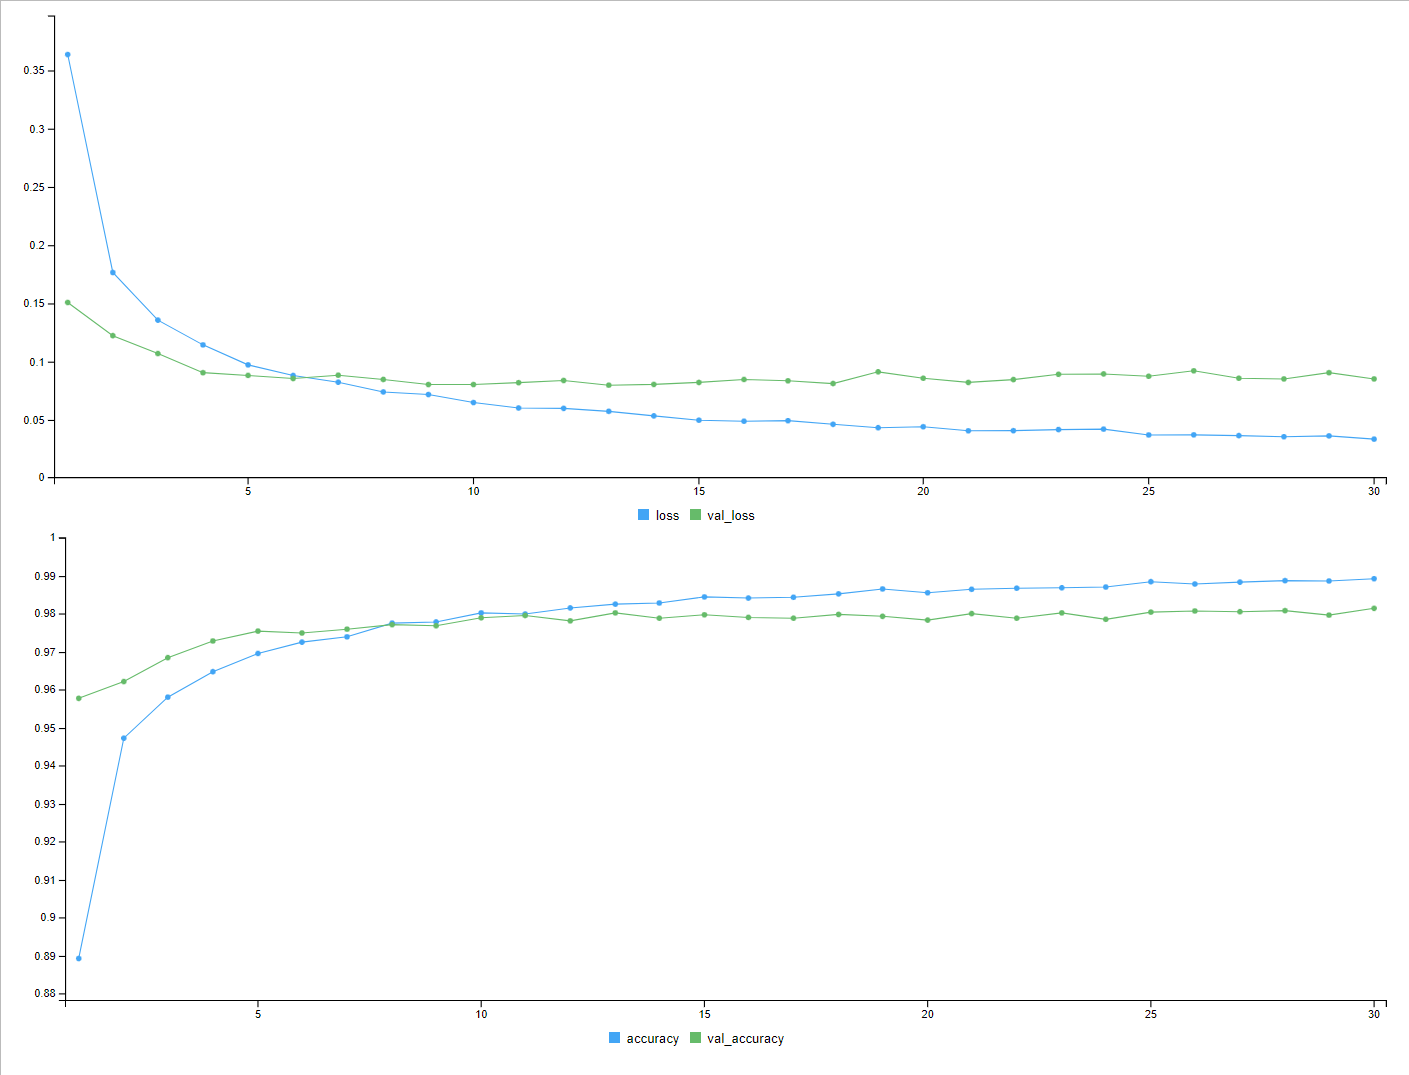
\includegraphics[width=\maxwidth]{Model2} \caption[Results for second model]{Results for second model}\label{fig:model2}
\end{figure}

\end{knitrout}

Looking at the results from the output as well as figure \ref{fig:model2}, then the accuracy is 98.9 and the validation accuracy is 0.982.


\subsection{1.5} If i were to use early stopping, then for each epoch we keep track of the parameter values as well as the accuracy.  Then in order to obtain a model with better validation error, I would return the parameter setting for the point in which the validation set accuracy was the highest.  If had do to implement it from scratch, then to the best of my knowledge I would have to write my own callback. But otherwise I probably can just use the defined method \texttt{Earlystopping} and something along the lines of:
\begin{knitrout}
\definecolor{shadecolor}{rgb}{0.969, 0.969, 0.969}\color{fgcolor}\begin{kframe}
\begin{alltt}
\hlstd{callback} \hlkwb{<-} \hlkwd{list}\hlstd{(}\hlkwd{callback_early_stopping}\hlstd{(}\hlkwc{patience} \hlstd{=} \hlnum{5}\hlstd{))}
\hlstd{history} \hlkwb{<-} \hlstd{model} \hlopt \hlkwd{fit}\hlstd{(}
  \hlcom{#rest of arguments here}
  \hlcom{#....}
  \hlkwc{callbacks} \hlstd{= callback}
\hlstd{)}
\end{alltt}
\end{kframe}
\end{knitrout}


\subsection{1.6}
For this task we want to find the best possible model. I tried to vary different arguments and parameters. In the end I just decided to stick with the following changes:
\begin{itemize}
\item Added 3 new hidden layers, each with relu activation and changed the number of units for all layers 
\item Added L\_2 regularizer for all hidden layers in order to apply penalties on layer parameters or layer activity during optimization. 
\item Specified that the images are in greyscale by adding 1 in input shape. But i do not know if it actually will affect performance.
\item Created a function \texttt{Scheduler()} to decrease the learning rate exponentially after 10 epochs
\item Implemented Early stopping.
\item increased batch size to 256
\end{itemize}

\begin{knitrout}
\definecolor{shadecolor}{rgb}{0.969, 0.969, 0.969}\color{fgcolor}\begin{kframe}
\begin{alltt}
\hlstd{model_best} \hlkwb{<-} \hlkwd{keras_model_sequential}\hlstd{()} \hlopt
  \hlkwd{layer_flatten}\hlstd{(}\hlkwc{input_shape} \hlstd{=} \hlkwd{c}\hlstd{(}\hlnum{28}\hlstd{,} \hlnum{28}\hlstd{,} \hlnum{1}\hlstd{))} \hlopt
  \hlkwd{layer_dense}\hlstd{(}\hlkwc{units} \hlstd{=} \hlnum{1024}\hlstd{,} \hlkwc{activation} \hlstd{=} \hlstr{'relu'}\hlstd{,}
              \hlkwc{kernel_regularizer} \hlstd{=} \hlkwd{regularizer_l2}\hlstd{(}\hlnum{0.001}\hlstd{))} \hlopt
  \hlkwd{layer_dropout}\hlstd{(}\hlnum{0.3}\hlstd{)} \hlopt
  \hlkwd{layer_batch_normalization}\hlstd{()} \hlopt
  \hlkwd{layer_dense}\hlstd{(}\hlkwc{units} \hlstd{=} \hlnum{512}\hlstd{,} \hlkwc{activation} \hlstd{=} \hlstr{'relu'}\hlstd{,}
              \hlkwc{kernel_regularizer} \hlstd{=} \hlkwd{regularizer_l2}\hlstd{(}\hlnum{0.001}\hlstd{))} \hlopt
  \hlkwd{layer_dropout}\hlstd{(}\hlnum{0.3}\hlstd{)} \hlopt
  \hlkwd{layer_batch_normalization}\hlstd{()} \hlopt
  \hlkwd{layer_dense}\hlstd{(}\hlkwc{units} \hlstd{=} \hlnum{256}\hlstd{,} \hlkwc{activation} \hlstd{=} \hlstr{'relu'}\hlstd{,}
              \hlkwc{kernel_regularizer} \hlstd{=} \hlkwd{regularizer_l2}\hlstd{(}\hlnum{0.001}\hlstd{))} \hlopt
  \hlkwd{layer_dropout}\hlstd{(}\hlnum{0.3}\hlstd{)} \hlopt
  \hlkwd{layer_batch_normalization}\hlstd{()} \hlopt
  \hlkwd{layer_dropout}\hlstd{(}\hlnum{0.3}\hlstd{)} \hlopt
   \hlkwd{layer_dense}\hlstd{(}\hlkwc{units}\hlstd{=}\hlnum{128}\hlstd{,} \hlkwc{activation}\hlstd{=}\hlstr{"relu"}\hlstd{,}
               \hlkwc{kernel_regularizer} \hlstd{=} \hlkwd{regularizer_l2}\hlstd{(}\hlnum{0.001}\hlstd{))} \hlopt
  \hlkwd{layer_batch_normalization}\hlstd{()} \hlopt
  \hlkwd{layer_dropout}\hlstd{(}\hlnum{0.3}\hlstd{)} \hlopt
   \hlkwd{layer_dense}\hlstd{(}\hlkwc{units}\hlstd{=}\hlnum{64}\hlstd{,} \hlkwc{activation}\hlstd{=}\hlstr{"relu"}\hlstd{,}
               \hlkwc{kernel_regularizer} \hlstd{=} \hlkwd{regularizer_l2}\hlstd{(}\hlnum{0.001}\hlstd{))} \hlopt
  \hlkwd{layer_batch_normalization}\hlstd{()} \hlopt
  \hlkwd{layer_dropout}\hlstd{(}\hlnum{0.3}\hlstd{)} \hlopt
  \hlkwd{layer_dense}\hlstd{(}\hlkwc{units} \hlstd{=} \hlnum{10}\hlstd{,} \hlkwc{activation} \hlstd{=} \hlstr{'softmax'}\hlstd{)}

\hlkwd{summary}\hlstd{(model_best)}
\end{alltt}
\begin{verbatim}
Model: "sequential_2"
________________________________________________________________________________
 Layer (type)                  Output Shape               Param #    Trainable  
================================================================================
 flatten_2 (Flatten)           (None, 784)                0          Y          
 dense_10 (Dense)              (None, 1024)               803840     Y          
 dropout_7 (Dropout)           (None, 1024)               0          Y          
 batch_normalization_6 (Batch  (None, 1024)               4096       Y          
 Normalization)                                                                 
 dense_9 (Dense)               (None, 512)                524800     Y          
 dropout_6 (Dropout)           (None, 512)                0          Y          
 batch_normalization_5 (Batch  (None, 512)                2048       Y          
 Normalization)                                                                 
 dense_8 (Dense)               (None, 256)                131328     Y          
 dropout_5 (Dropout)           (None, 256)                0          Y          
 batch_normalization_4 (Batch  (None, 256)                1024       Y          
 Normalization)                                                                 
 dropout_4 (Dropout)           (None, 256)                0          Y          
 dense_7 (Dense)               (None, 128)                32896      Y          
 batch_normalization_3 (Batch  (None, 128)                512        Y          
 Normalization)                                                                 
 dropout_3 (Dropout)           (None, 128)                0          Y          
 dense_6 (Dense)               (None, 64)                 8256       Y          
 batch_normalization_2 (Batch  (None, 64)                 256        Y          
 Normalization)                                                                 
 dropout_2 (Dropout)           (None, 64)                 0          Y          
 dense_5 (Dense)               (None, 10)                 650        Y          
================================================================================
Total params: 1509706 (5.76 MB)
Trainable params: 1505738 (5.74 MB)
Non-trainable params: 3968 (15.50 KB)
________________________________________________________________________________
\end{verbatim}
\end{kframe}
\end{knitrout}

\begin{knitrout}
\definecolor{shadecolor}{rgb}{0.969, 0.969, 0.969}\color{fgcolor}\begin{kframe}
\begin{alltt}
\hlstd{model_best} \hlopt \hlkwd{compile}\hlstd{(}
  \hlkwc{optimizer} \hlstd{=} \hlstr{'RMSprop'}\hlstd{,}
  \hlkwc{loss} \hlstd{=} \hlstr{'categorical_crossentropy'}\hlstd{,}
  \hlkwc{metrics} \hlstd{=} \hlkwd{c}\hlstd{(}\hlstr{'accuracy'}\hlstd{)}
\hlstd{)}


\hlstd{Scheduler} \hlkwb{<-} \hlkwa{function}\hlstd{(}\hlkwc{epoch}\hlstd{,} \hlkwc{lr}\hlstd{) \{}
  \hlkwa{if} \hlstd{(epoch} \hlopt{<} \hlnum{15}\hlstd{) \{}
    \hlkwd{return}\hlstd{(lr)}
  \hlstd{\}} \hlkwa{else} \hlstd{\{}
    \hlkwd{return}\hlstd{(lr} \hlopt{*} \hlkwd{exp}\hlstd{(}\hlopt{-}\hlnum{0.1}\hlstd{))}
  \hlstd{\}}
\hlstd{\}}

\hlstd{callback_list} \hlkwb{=} \hlkwd{list}\hlstd{(}\hlkwd{callback_early_stopping}\hlstd{(}\hlkwc{patience} \hlstd{=} \hlnum{10}\hlstd{),}
                     \hlkwd{callback_learning_rate_scheduler}\hlstd{(Scheduler))}

\hlstd{history} \hlkwb{<-} \hlstd{model_best} \hlopt \hlkwd{fit}\hlstd{(}
  \hlstd{x_train, y_train,}
  \hlkwc{epochs} \hlstd{=} \hlnum{75}\hlstd{,}\hlkwc{batch_size} \hlstd{=} \hlnum{256}\hlstd{,}
  \hlkwc{validation_split} \hlstd{=} \hlnum{0.2}\hlstd{,}
  \hlkwc{callbacks} \hlstd{=callback_list,}
  \hlkwc{verbose} \hlstd{=} \hlnum{1}\hlstd{)}
\end{alltt}
\end{kframe}
\end{knitrout}
This terminated early at epoch 59 with the following result:

\begin{knitrout}
\definecolor{shadecolor}{rgb}{0.969, 0.969, 0.969}\color{fgcolor}\begin{kframe}
\begin{alltt}
Epoch 59/75
188/188 [==============================] - 7s 40ms/step 
- loss: 0.0368 - accuracy: 0.9977 - val_loss: 0.1097 - val_accuracy: 0.9854 - lr: 1.2277e-05
\end{alltt}
\end{kframe}
\end{knitrout}
However, since it used early stopping, I am not sure about which epoch exactly it decided on in the end. Either wait, the accuracy is around 0.997 and the validation accuracy is around 0.985. The results can also be seen in figure \ref{fig:model3} below:
\begin{knitrout}
\definecolor{shadecolor}{rgb}{0.969, 0.969, 0.969}\color{fgcolor}\begin{kframe}
\begin{alltt}
\hlstd{knitr}\hlopt{::}\hlkwd{include_graphics}\hlstd{(}\hlstr{"model3.png"}\hlstd{)}
\end{alltt}
\end{kframe}\begin{figure}
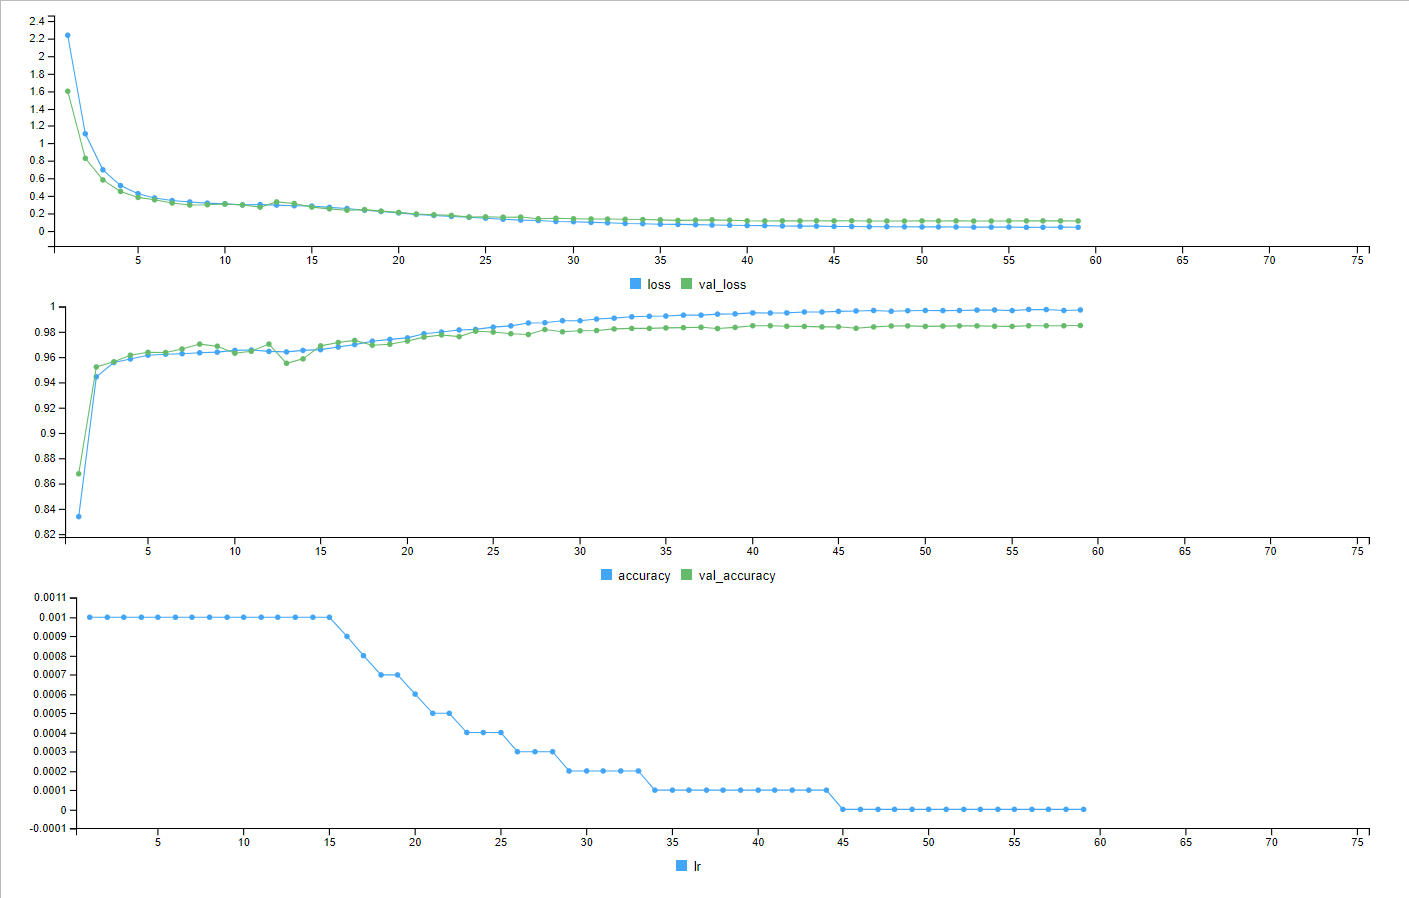
\includegraphics[width=\maxwidth]{model3} \caption[Results for the third model]{Results for the third model}\label{fig:model3}
\end{figure}

\end{knitrout}



\subsection{1.7}
Now we identify two digits that the network has classified incorrectly. 
\begin{knitrout}
\definecolor{shadecolor}{rgb}{0.969, 0.969, 0.969}\color{fgcolor}\begin{kframe}
\begin{alltt}
\hlstd{predictions} \hlkwb{<-} \hlstd{model_best} \hlopt \hlkwd{predict}\hlstd{(x_test)}
\hlstd{predicted_labels} \hlkwb{<-} \hlkwd{max.col}\hlstd{(predictions)} \hlopt{-} \hlnum{1}
\hlstd{true_labels} \hlkwb{<-} \hlkwd{max.col}\hlstd{(y_test)} \hlopt{-} \hlnum{1}
\hlcom{# Gives the column for which the number is 1, which corresponds to the digit.}
\hlcom{#  subtract 1 since numbers   starts at 0}


\hlstd{incorrect_indices} \hlkwb{<-} \hlkwd{which}\hlstd{(predicted_labels} \hlopt{!=} \hlstd{true_labels)}

\hlstd{incorrect_images} \hlkwb{<-} \hlstd{x_test[incorrect_indices, ,]}

\hlkwd{plot_images}\hlstd{(}\hlkwc{image_array} \hlstd{= x_test, ,} \hlkwc{y}\hlstd{=mnist}\hlopt{$}\hlstd{test}\hlopt{$}\hlstd{y,}\hlkwc{pred} \hlstd{= predicted_labels,}
            \hlkwc{idx} \hlstd{= incorrect_indices[}\hlnum{1}\hlopt{:}\hlnum{8}\hlstd{])}
\hlcom{#they look really scuffed}
\end{alltt}
\end{kframe}
\end{knitrout}

\begin{knitrout}
\definecolor{shadecolor}{rgb}{0.969, 0.969, 0.969}\color{fgcolor}\begin{kframe}
\begin{alltt}
\hlstd{knitr}\hlopt{::}\hlkwd{include_graphics}\hlstd{(}\hlstr{"wrong_preds.png"}\hlstd{)}
\end{alltt}
\end{kframe}\begin{figure}
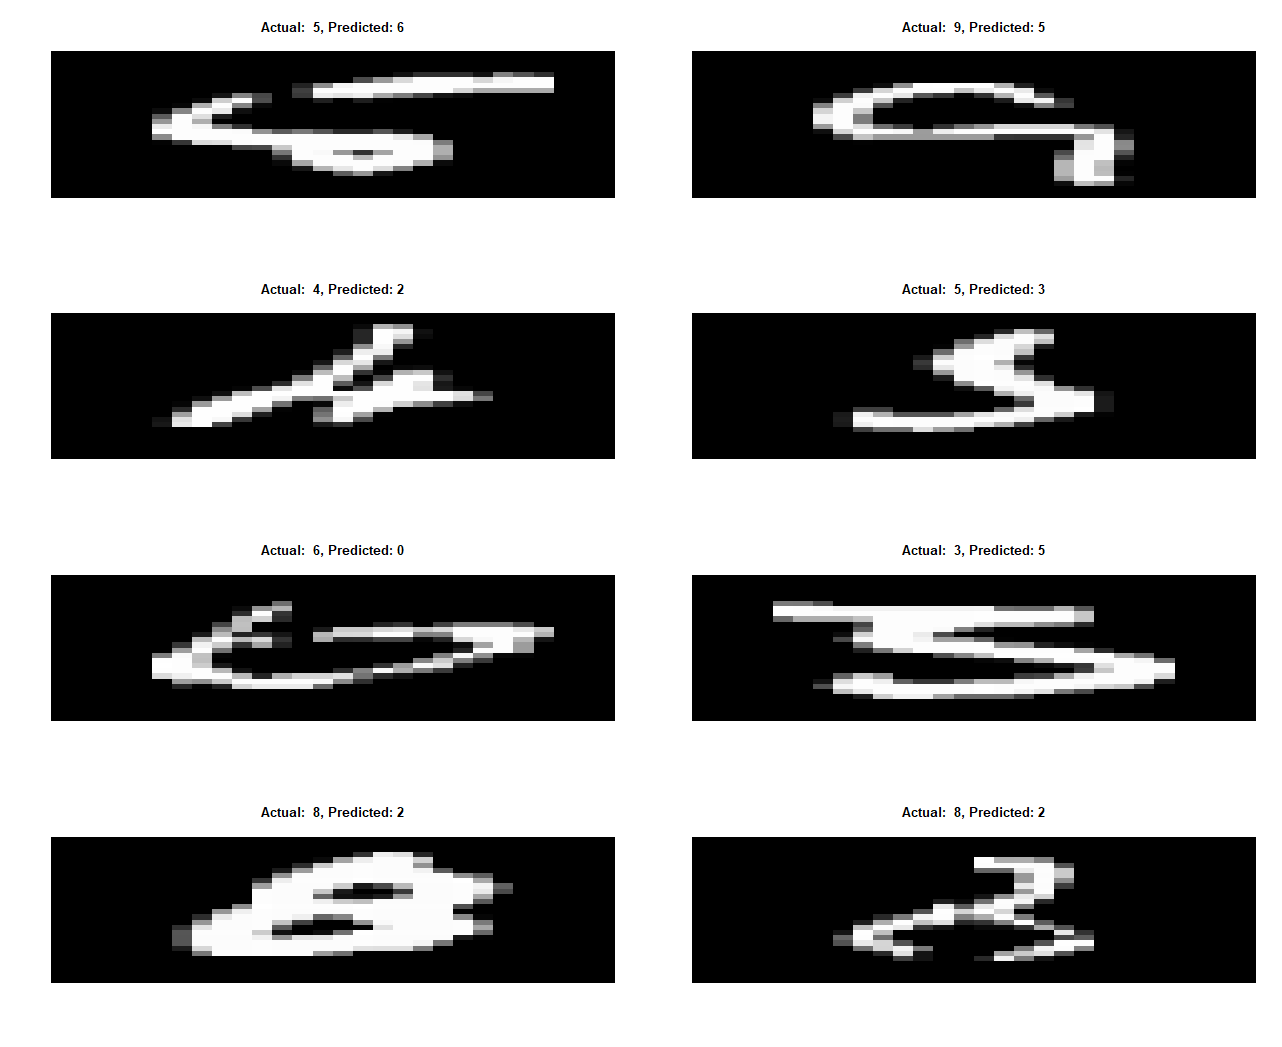
\includegraphics[width=\maxwidth]{wrong_preds} \caption[Actual and predicted values for wrongly classified images]{Actual and predicted values for wrongly classified images}\label{fig:preds}
\end{figure}

\end{knitrout}

Figure \ref{fig:preds} shows the some of the wrongly classified images with the predicted values above each image. Looking at them, Then based on the images i would say its not really that surprising seeing as some of them look really scuffed and even I cannot really tell what some of them are supposed to be just by looking at them.

\subsection{1.8}
Now we compute the accuracy on the hold-out test set.
\begin{knitrout}
\definecolor{shadecolor}{rgb}{0.969, 0.969, 0.969}\color{fgcolor}\begin{kframe}
\begin{alltt}
model_best %>% \hlkwd{evaluate}(x_test, y_test)

13/313 [==============================] - 1s 4ms/step - loss: 0.1017 - accuracy: 0.9866
     loss  accuracy 
0.1017455 0.9866000 
\end{alltt}
\end{kframe}
\end{knitrout}

 
 It seems that it is  0.987, which is around the as the validation accuracy from the model when training it. I would say it makes sense in overall since the validation accuracy is supposed to be the sample that is not used in the training for each epoch. However, it is still lower than the normal accuracy at 99.7 percent, which could indicate some overfitting with respect to the whole training model. However, in my opinion, the test accuracy is still rather close so it should not be of any major concern. Perhaps the accuracy could also be explained partly due to the images being very similar to each other, and thus for the most part the model could easily be applied on the test data as well. 

 
 \subsection{Task 2}
 \subsection{2.1}
\begin{knitrout}
\definecolor{shadecolor}{rgb}{0.969, 0.969, 0.969}\color{fgcolor}\begin{kframe}
\begin{alltt}
\hlstd{W} \hlkwb{<-} \hlkwd{matrix}\hlstd{(}\hlnum{1}\hlstd{,} \hlkwc{nrow} \hlstd{=} \hlnum{2}\hlstd{,} \hlkwc{ncol} \hlstd{=} \hlnum{2}\hlstd{)}
\hlstd{c} \hlkwb{<-} \hlkwd{matrix}\hlstd{(}\hlkwd{c}\hlstd{(}\hlnum{0}\hlstd{,} \hlopt{-}\hlnum{1}\hlstd{) ,} \hlkwc{ncol} \hlstd{=} \hlnum{2}\hlstd{,} \hlkwc{nrow} \hlstd{=} \hlnum{4}\hlstd{,} \hlkwc{byrow} \hlstd{=} \hlnum{TRUE}\hlstd{)}
\hlstd{X} \hlkwb{<-} \hlkwd{matrix}\hlstd{(}\hlkwd{c}\hlstd{(}\hlnum{0}\hlstd{,} \hlnum{0}\hlstd{,} \hlnum{1}\hlstd{,} \hlnum{1}\hlstd{,} \hlnum{0}\hlstd{,} \hlnum{1}\hlstd{,} \hlnum{0}\hlstd{,} \hlnum{1}\hlstd{),} \hlkwc{ncol} \hlstd{=} \hlnum{2}\hlstd{)}
\hlstd{w} \hlkwb{<-} \hlkwd{matrix}\hlstd{(}\hlkwd{c}\hlstd{(}\hlnum{1}\hlstd{,} \hlopt{-}\hlnum{2}\hlstd{) ,} \hlkwc{ncol} \hlstd{=} \hlnum{1}\hlstd{)}
\hlstd{b} \hlkwb{<-} \hlnum{0}

\hlstd{RLF} \hlkwb{<-} \hlkwa{function}\hlstd{(}\hlkwc{i}\hlstd{)} \hlkwd{return}\hlstd{(}\hlkwd{max}\hlstd{(}\hlnum{0}\hlstd{,i))}

\hlstd{mini_net} \hlkwb{<-} \hlkwa{function}\hlstd{(}\hlkwc{X}\hlstd{,} \hlkwc{W}\hlstd{,} \hlkwc{c}\hlstd{,} \hlkwc{w}\hlstd{,} \hlkwc{b}\hlstd{)\{}

  \hlstd{RLF_input} \hlkwb{<-}  \hlstd{X}\hlopt\hlstd{W} \hlopt{+} \hlstd{c}
 \hlstd{transformed_res}  \hlkwb{<-} \hlkwd{apply}\hlstd{(RLF_input,} \hlkwc{MARGIN} \hlstd{=} \hlkwd{c}\hlstd{(}\hlnum{1}\hlstd{,}\hlnum{2}\hlstd{),} \hlkwc{FUN}\hlstd{= RLF)}

  \hlkwd{return}\hlstd{(transformed_res} \hlopt \hlstd{w} \hlopt{+} \hlstd{b)}
\hlstd{\}}
\end{alltt}
\end{kframe}
\end{knitrout}

\begin{knitrout}
\definecolor{shadecolor}{rgb}{0.969, 0.969, 0.969}\color{fgcolor}\begin{kframe}
\begin{alltt}
\hlkwd{mini_net}\hlstd{(X, W, c, w, b)}
\end{alltt}
\begin{verbatim}
     [,1]
[1,]    0
[2,]    1
[3,]    1
[4,]    0
\end{verbatim}
\begin{alltt}
\hlkwd{mini_net}\hlstd{(X, W}\hlopt{*}\hlnum{0.9}\hlstd{, c, w, b)}
\end{alltt}
\begin{verbatim}
     [,1]
[1,]  0.0
[2,]  0.9
[3,]  0.9
[4,]  0.2
\end{verbatim}
\end{kframe}
\end{knitrout}
 
 \subsection{2.2}
 Now we change $W_{1,1}$ to 0.
 
\begin{knitrout}
\definecolor{shadecolor}{rgb}{0.969, 0.969, 0.969}\color{fgcolor}\begin{kframe}
\begin{alltt}
\hlstd{W[}\hlnum{1}\hlstd{,}\hlnum{1}\hlstd{]}\hlkwb{<-} \hlnum{0}

\hlkwd{mini_net}\hlstd{(X, W, c, w, b)}
\end{alltt}
\begin{verbatim}
     [,1]
[1,]    0
[2,]    1
[3,]    0
[4,]   -1
\end{verbatim}
\begin{alltt}
\hlkwd{mini_net}\hlstd{(X, W}\hlopt{*}\hlnum{0.9}\hlstd{, c, w, b)}
\end{alltt}
\begin{verbatim}
     [,1]
[1,]  0.0
[2,]  0.9
[3,]  0.0
[4,] -0.7
\end{verbatim}
\end{kframe}
\end{knitrout}
 \subsection{2.3}
 The current output functions is a linear function, but the first part captures the nonlinear information so I think its still reasonable. However, perhaps one could consider something else such as the sigmoid function since it is suitable for 0-1 binary values. 
 \subsection{2.4}
 Now we implement a squared loss function.
\begin{knitrout}
\definecolor{shadecolor}{rgb}{0.969, 0.969, 0.969}\color{fgcolor}\begin{kframe}
\begin{alltt}
\hlstd{XOR} \hlkwb{<-} \hlkwa{function}\hlstd{(}\hlkwc{x1}\hlstd{,} \hlkwc{x2}\hlstd{)\{}
  \hlkwa{if}\hlstd{(x1} \hlopt{==}\hlnum{1} \hlopt{&} \hlstd{x2}\hlopt{!=}\hlnum{1} \hlopt{|} \hlstd{x1}\hlopt{!=} \hlnum{1} \hlopt{&} \hlstd{x2} \hlopt{==}\hlnum{1}\hlstd{)\{}
  \hlkwd{return}\hlstd{(}\hlnum{1}\hlstd{)\}} \hlkwa{else}\hlstd{\{}
    \hlkwd{return}\hlstd{(}\hlnum{0}\hlstd{)}
  \hlstd{\}}
\hlstd{\}}

\hlcom{#changing W back to original values }
\hlstd{W} \hlkwb{<-} \hlkwd{matrix}\hlstd{(}\hlnum{1}\hlstd{,} \hlkwc{nrow} \hlstd{=} \hlnum{2}\hlstd{,} \hlkwc{ncol} \hlstd{=} \hlnum{2}\hlstd{)}
\hlstd{mini_net_loss} \hlkwb{<-} \hlkwa{function}\hlstd{(}\hlkwc{X}\hlstd{,} \hlkwc{W}\hlstd{,} \hlkwc{c}\hlstd{,} \hlkwc{w}\hlstd{,} \hlkwc{b}\hlstd{)\{}
  \hlstd{mini_res} \hlkwb{<-} \hlkwd{mini_net}\hlstd{(X, W, c, w, b)}
\hlstd{xor_res} \hlkwb{<-} \hlkwd{apply}\hlstd{(X,} \hlkwc{MARGIN}\hlstd{=}\hlnum{1}\hlstd{,} \hlkwc{FUN}\hlstd{=}\hlkwa{function}\hlstd{(}\hlkwc{row}\hlstd{)\{} \hlkwd{XOR}\hlstd{(row[}\hlnum{1}\hlstd{], row[}\hlnum{2}\hlstd{])\})}
\hlstd{summand} \hlkwb{<-} \hlkwd{sum}\hlstd{((xor_res} \hlopt{-}\hlstd{mini_res)}\hlopt{^}\hlnum{2}\hlstd{)}
\hlstd{average} \hlkwb{<-} \hlstd{summand} \hlopt{/} \hlkwd{nrow}\hlstd{(X)}
\hlkwd{return}\hlstd{(average)}
\hlstd{\}}

\hlkwd{mini_net_loss}\hlstd{(X, W, c, w, b)}
\end{alltt}
\begin{verbatim}
[1] 0
\end{verbatim}
\begin{alltt}
\hlkwd{mini_net_loss}\hlstd{(X,} \hlnum{0.9}\hlopt{*}\hlstd{W, c, w, b)}
\end{alltt}
\begin{verbatim}
[1] 0.015
\end{verbatim}
\begin{alltt}
\hlcom{## Originally I did not see it was supposed to be with a given Y argument,}
\hlcom{#but since i already implemented the abvove one, we might as well just compare }
\hlcom{#the results. }
\hlstd{mini_net_loss_2}\hlkwb{<-} \hlkwa{function}\hlstd{(}\hlkwc{y}\hlstd{,} \hlkwc{X}\hlstd{,} \hlkwc{W}\hlstd{,} \hlkwc{c}\hlstd{,} \hlkwc{w}\hlstd{,} \hlkwc{b}\hlstd{)\{}
  \hlstd{mini_res} \hlkwb{<-} \hlkwd{mini_net}\hlstd{(}\hlkwc{X}\hlstd{=X,} \hlkwc{W}\hlstd{=W,} \hlkwc{c}\hlstd{=c,} \hlkwc{w}\hlstd{=w,} \hlkwc{b}\hlstd{=b)}
  \hlstd{summand} \hlkwb{<-} \hlkwd{sum}\hlstd{((y}\hlopt{-}\hlstd{mini_res)}\hlopt{^}\hlnum{2}\hlstd{)}
  \hlstd{average} \hlkwb{<-} \hlstd{summand}\hlopt{/}\hlkwd{nrow}\hlstd{(X)}
  \hlkwd{return}\hlstd{(average)}
\hlstd{\}}

\hlstd{y} \hlkwb{<-} \hlkwd{c}\hlstd{(}\hlnum{0}\hlstd{,} \hlnum{1}\hlstd{,} \hlnum{1}\hlstd{,} \hlnum{0}\hlstd{)}
\hlkwd{mini_net_loss_2}\hlstd{(y, X, W, c, w, b)}
\end{alltt}
\begin{verbatim}
[1] 0
\end{verbatim}
\begin{alltt}
\hlkwd{mini_net_loss_2}\hlstd{(y, X,} \hlnum{0.9}\hlopt{*}\hlstd{W, c, w, b)}
\end{alltt}
\begin{verbatim}
[1] 0.015
\end{verbatim}
\end{kframe}
\end{knitrout}

\subsection{2.5}
\begin{knitrout}
\definecolor{shadecolor}{rgb}{0.969, 0.969, 0.969}\color{fgcolor}\begin{kframe}
\begin{alltt}
\hlcom{#change W[1,1] again}
\hlstd{W[}\hlnum{1}\hlstd{,}\hlnum{1}\hlstd{]} \hlkwb{<-} \hlnum{0}

\hlkwd{mini_net_loss}\hlstd{(X, W, c, w, b)}
\end{alltt}
\begin{verbatim}
[1] 0.5
\end{verbatim}
\begin{alltt}
\hlkwd{mini_net_loss_2}\hlstd{(y, X, W, c, w, b)}
\end{alltt}
\begin{verbatim}
[1] 0.5
\end{verbatim}
\begin{alltt}
\hlkwd{mini_net_loss}\hlstd{(X,} \hlnum{0.9}\hlopt{*}\hlstd{W, c, w, b)}
\end{alltt}
\begin{verbatim}
[1] 0.375
\end{verbatim}
\begin{alltt}
\hlkwd{mini_net_loss_2}\hlstd{(y, X,} \hlnum{0.9}\hlopt{*}\hlstd{W, c, w, b)}
\end{alltt}
\begin{verbatim}
[1] 0.375
\end{verbatim}
\end{kframe}
\end{knitrout}
 
\end{document}



@


@
